\documentclass[UTF8]{ctexart}
\usepackage{geometry, CJKutf8}
\geometry{margin=1.5cm, vmargin={0pt,1cm}}
\setlength{\topmargin}{-1cm}
\setlength{\paperheight}{29.7cm}
\setlength{\textheight}{25.3cm}

% useful packages.
\usepackage{amsfonts}
\usepackage{graphicx}
\usepackage{amsmath}
\usepackage{amssymb}
\usepackage{amsthm}
\usepackage{enumerate}
\usepackage{graphicx}
\usepackage{multicol}
\usepackage{fancyhdr}
\usepackage{layout}
\usepackage{listings}
\usepackage{float, caption}
\usepackage{titling}

\pretitle{\begin{center}\Huge\bfseries}
\posttitle{\end{center}}
\preauthor{\begin{center}\Large\scshape}
\postauthor{\end{center}}
\predate{\begin{center}\large}
\postdate{\end{center}}

\lstset{
    basicstyle=\ttfamily, basewidth=0.5em
}

% some common command
\newcommand{\dif}{\mathrm{d}}
\newcommand{\avg}[1]{\left\langle #1 \right\rangle}
\newcommand{\difFrac}[2]{\frac{\dif #1}{\dif #2}}
\newcommand{\pdfFrac}[2]{\frac{\partial #1}{\partial #2}}
\newcommand{\OFL}{\mathrm{OFL}}
\newcommand{\UFL}{\mathrm{UFL}}
\newcommand{\fl}{\mathrm{fl}}
\newcommand{\op}{\odot}
\newcommand{\Eabs}{E_{\mathrm{abs}}}
\newcommand{\Erel}{E_{\mathrm{rel}}}

\setlength{\droptitle}{-1cm}

\title{作业报告}
\author{自动化(控制) 韩 箫;3230100653}
\date{2024.10.20}

\begin{document}

\maketitle

\pagestyle{fancy}
\fancyhead{}
\lhead{韩箫, 32301000653}
\chead{数据结构与算法第四次作业}
\rhead{Oct.20th, 2024}


\section{测试程序的设计思路}
\begin{enumerate}
    \item 使用初始化列表构造函数和拷贝构造函数,来创建多个 List 对象,并打印每个 List 对象的内容,直接观察验证构造函数的正确性。
    \item 使用赋值运算符,将一个 List 对象赋值给另一个 List 对象。打印赋值后的 List 对象的内容,验证重载后的拷贝赋值函数。并进行连续赋值,验证拷贝复制的返回情况是否正确。再进行自身赋值,检验正确性。
    \item 调用移动构造函数,使用 std::move 将一个 List 对象移动到另一个 List 对象,输出内容来验证移动构造函数的正确性。同理进行移动赋值的测试。
    \item 调用 push函数,实则也对内嵌的insert函数进行了调用和检验。
    \item 使用 pop方法从 List 对象的前后删除元素,同理也同时检验了remove 函数。
    \item 使用 front 和 back 方法访问已知对象的第一个和最后一个元素,直接观察判断检验。
    \item 使用 clear 方法清空 List 对象,并打印空列表进行检验。
    \item 使用 isEmpty 方法检查预先已知的一个空链表和一个非空链表,观察结果是否符合预期。
    \item 使用 getsize 方法获取一个已知表的大小。
    \item 最后调用析构函数进行清理,并为防止重复清理增加判断和报错。
\end{enumerate}


\section{测试结果}
测试结果如图 \ref{fig:result} 所示,测试结果正常,符合直观预期。
\begin{figure}[h]
    \centering
    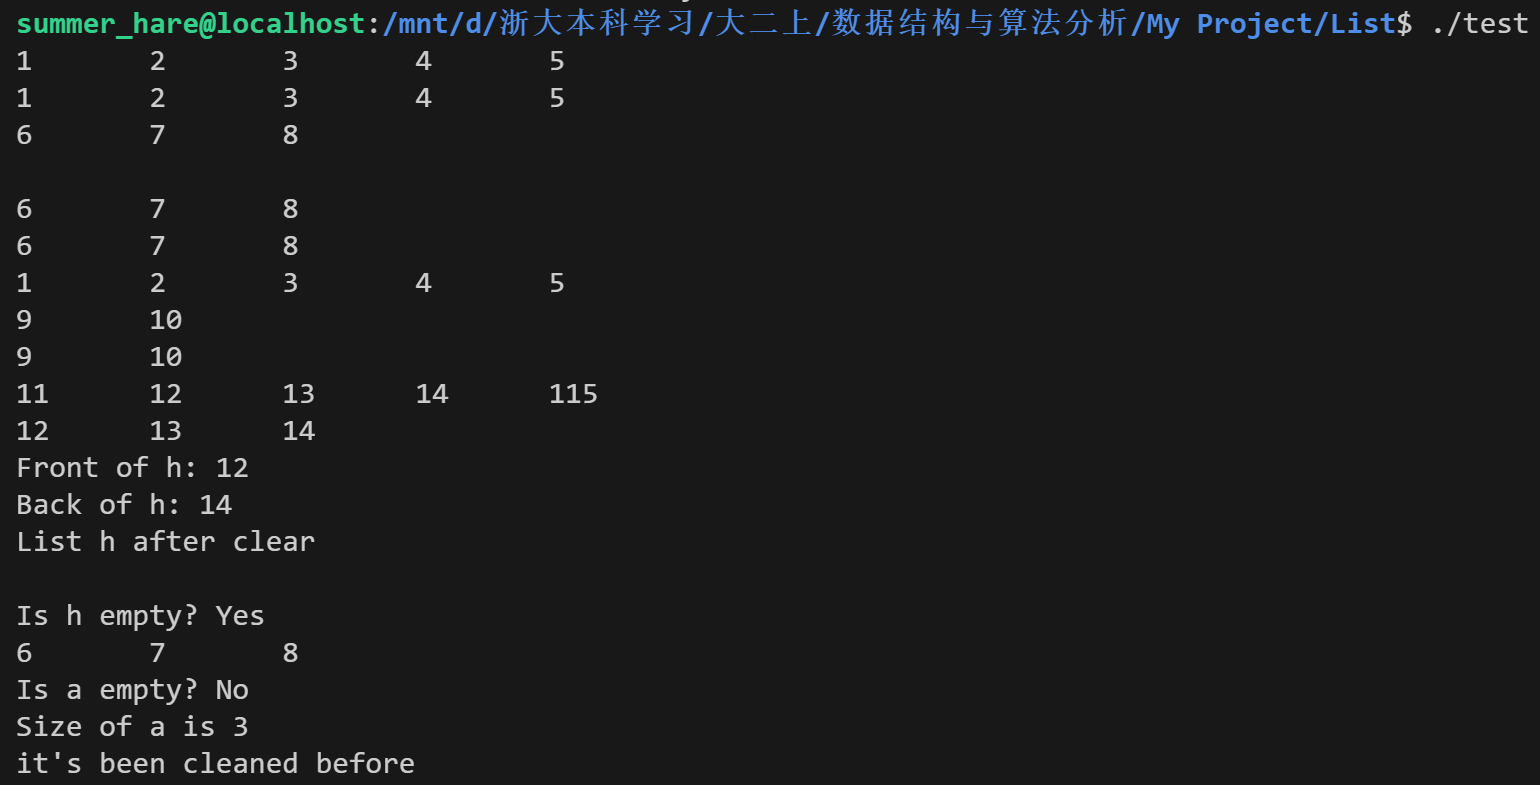
\includegraphics[width=0.8\textwidth]{运行结果.png} 
    \caption{测试结果}
    \label{fig:result}
\end{figure}


我用 valgrind 进行测试,发现没有发生内存泄露。
测试报告如图 \ref{fig:valgrind} 所示
\begin{figure}[h]
    \centering
    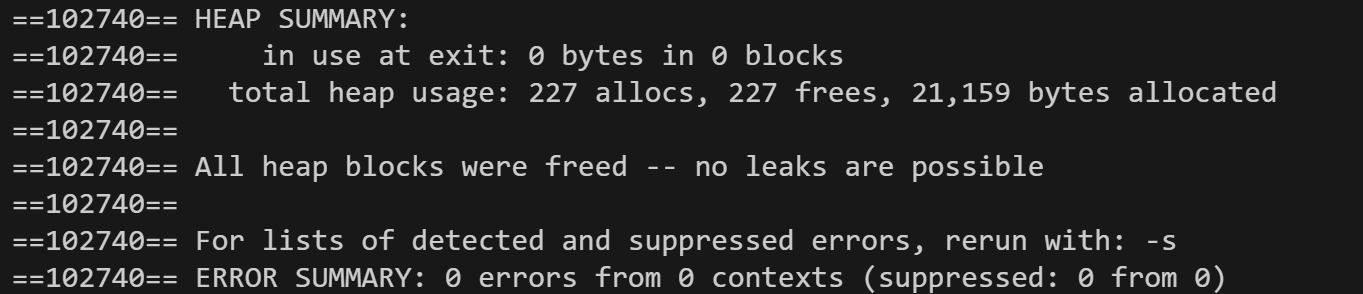
\includegraphics[width=0.8\textwidth]{内存泄漏检查.png} 
    \caption{valgrind 测试报告}
    \label{fig:valgrind}
\end{figure}

\section{bug报告}

我发现了一个 bug,触发条件如下:

\begin{enumerate}
    \item 如果不在clear以及remove函数中增加对head和tail情况的判断和相应报错,在析构函数中会重复释放内存,导致Segmentation fault,如图 \ref{fig:error}所示。
    \begin{figure}[h]
        \centering
        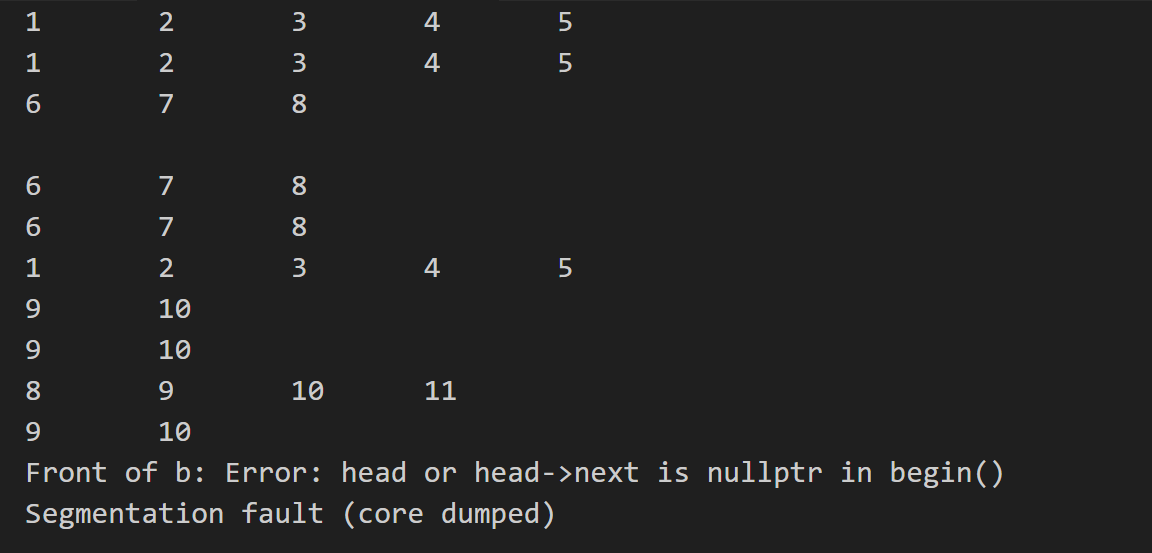
\includegraphics[width=0.8\textwidth]{Segmentaion fault.png} 
        \caption{Segmentation fault}
        \label{fig:error}
    \end{figure}
    \item 通过我在begin函数中所加的报错语句,可见此时有head指针变为了空指针。而教材中目前授课进度所涉及的部分还未包含错误检验。所以若完全遵照教材代码,就会出现该问题。
    \item 如果在clear函数中增加检验和反馈的语句,如图 \ref{fig:test} 所示,会发现在remove函数中的head和tail已经被清理,因此导致重复释放内存。
    \begin{figure}[h]
        \centering
        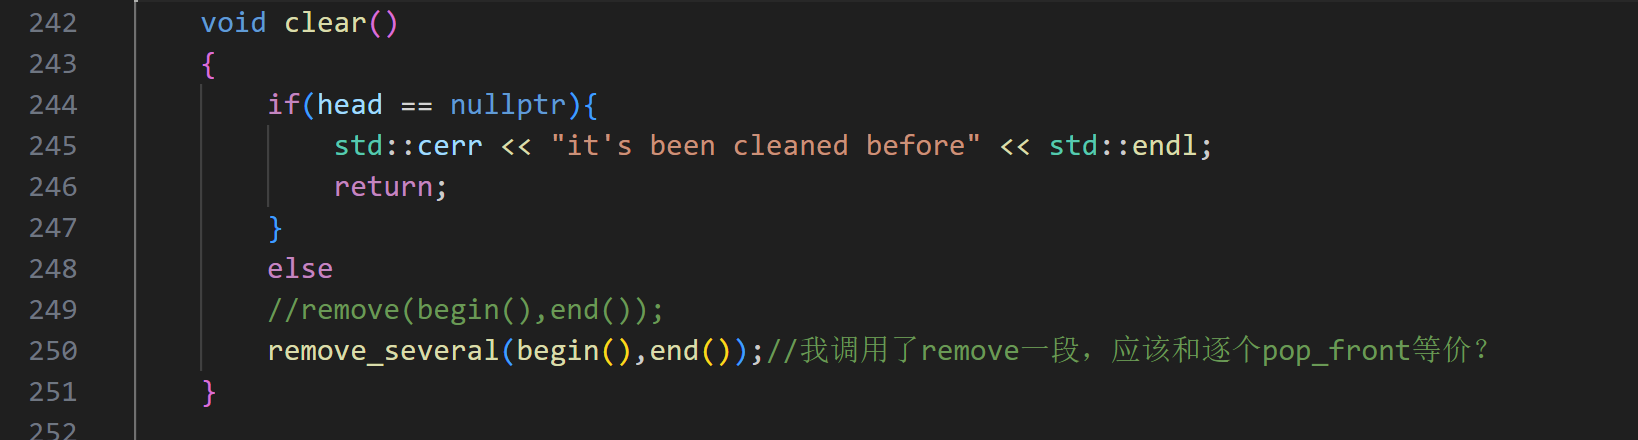
\includegraphics[width=0.8\textwidth]{报错语句.png} 
        \caption{clear 检验}
        \label{fig:test}
    \end{figure}

\end{enumerate}

\subsection{原因分析}
\begin{enumerate}
    \item 如前所述,在begin函数中增加了报错语句,可以看到head指针变为了空指针,但在remove函数中没有对这种情况进行相应的处理。
    \item 经过后来的调试,发现程序在输出 a.getsize() 之后应该已经完成了所有的操作,但仍然出现了 segmentation fault。这可能是由于程序在退出时调用了某些析构函数,而这些析构函数中可能存在对无效指针的访问。
    即在主程序所有的显式的函数都完成调用之后,仍然会发生begin的报错,由此推断应当是析构函数的问题。因为只有析构函数在所有显式的函数调用完成后还会被调用。
    \item 确定析构函数后再倒推,可能是移动后的对象状态:在调用 std::move 后,原对象的状态是未定义的。
    \item 在调用 std::move(b) 后,b 的状态确实是未定义的,因此不应该再使用该链表。同时为了防止错误,应当在代码中添加检查,在访问之前确认其状态。
\end{enumerate}
\subsection{解决方法}
    所以最终我在remove以及clear中加上了相应的判断和检验语句,如图 \ref{fig:test},问题得到解决。

\section{代码细节改动或改进}
    因为是自己写了一遍完整的代码,所以有一些地方和教材会有一定出入和改动,再此罗列说明。
\begin{enumerate}
    \item 初始化函数initialization中,如果不对iterator的current指针进行相应的初始化,可能会为空,或者原有内容清空后变为未定义,是否会引发一些错误?
    因此增加了初始化current为tail的语句,如图 \ref{fig:initialize},之所以将current初始化为tail而非head,主要是因为考虑insert函数是在current所指节点之前插入新节点。
    \begin{figure}[h]
        \centering
        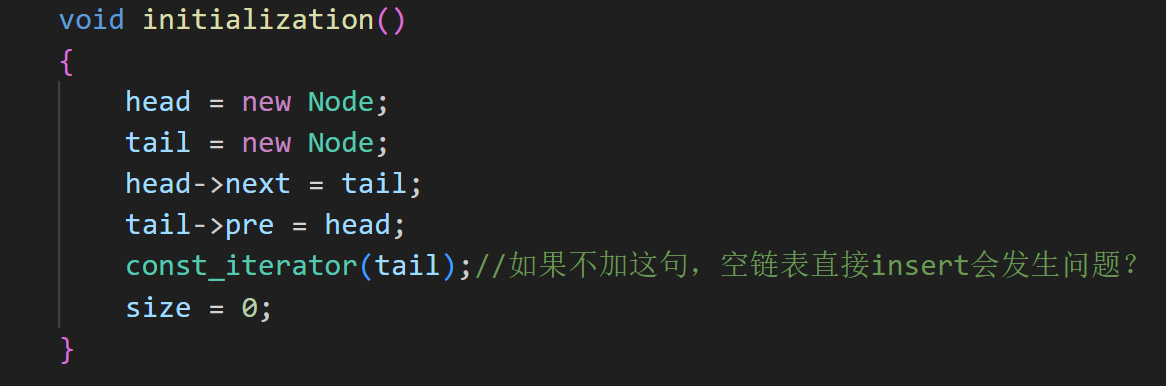
\includegraphics[width=0.8\textwidth]{初始化current.png} 
        \caption{初始化current}
        \label{fig:initialize}
    \end{figure}

    \item 另外,经过编译发现,如果按教材代码所写,不明确指出所用的current是在哪个迭代器之下,编译器也会报错,如图 \ref{fig:iterator} 所示。所以在自增等几个迭代器函数中都明确写了this->current,证明实际操作与教材仍存在差异性。
    \begin{figure}[h]
        \centering
        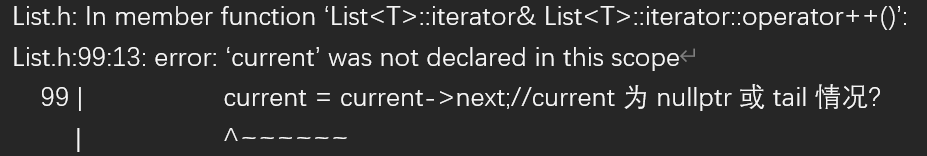
\includegraphics[width=0.8\textwidth]{current归属.png} 
        \caption{current归属}
        \label{fig:iterator}
    \end{figure}

    \item 要求思考remove一串节点的情况,内外循环的逻辑相似,可以进行优化,因此我在LIst.h的line214-234写了另一个版本的remove-several函数,和remove单个节点的逻辑略有不同,应该能减少一些指针操作?
    \item 在clear函数中,教材代码给的是while循环下的pop-front函数,我直接使用了remove-several函数,经过测试检验效果应该是等价的。
    \item 关于push和pop函数,本身内在逻辑是调用insert和remove函数;但insert和remove函数本身已经定义了左值和右值两种版本,所以push和pop函数左值和右值版本,好像也没有必要再调用move函数对参数进行转换,结果来看是等价的。
    \item 移动赋值函数似乎没有被拷贝赋值所替代,不写的话还是会报错,和课上讲得有出入?所以还是写了一下,另外教材代码中的赋值都没有对自身赋值进行判断,所以我都加了一句判断。
\end{enumerate}
\subsection{初学者水平有限,不当修改之处和不完善的想法,恳请指正包涵}

\section{附记部分心得和细节总结}
    因为感觉对数据结构和C++语言本身不是很熟悉,所以还是自己写了一遍完整的程序,以期有更深入的记忆和感觉。在这个过程中,确实一点一点打代码,会比直接看教材代码,对于细节会有更多的关注和思考。通过和gpt的讨论,对一些知识细节有了更深入的理解。
    让gpt基于对话问答生成了一份知识点总结,下附于此。
    \begin{itemize}  
        \item \textbf{迭代器的 operator++() 中 *this 返回值是什么?}  
          
        在迭代器的 operator++() 方法中,return *this 返回的是调用 operator++() 这个函数的对象本身,而不仅仅是 current 成员。这是因为 this 是一个指向当前对象的指针,*this 就是这个对象本身。当你执行 current = current->next; 后,你改变了对象的 current 成员,但这个对象可能还有其他的成员。  
          
        \item \textbf{迭代器的 * 操作符为什么不直接返回节点?}  
          
        迭代器的 * 操作符通常用来获取当前迭代器指向的元素的值,而不是获取迭代器本身或者底层的节点。这是因为迭代器的设计目的是为了让用户能够方便地访问和遍历容器中的元素,而不需要关心底层的实现细节。  
          
        \item \textbf{函数参数的左值和右值输入?}  
          
        如果函数的参数是一个普通类型(非引用类型),那么无论你传入的是左值还是右值,都可以正常调用。但是,如果函数的参数是一个引用类型,那么情况就会有所不同。如果参数是一个非常量左值引用,那么你只能传入左值。如果参数是一个常量左值引用,那么你可以传入左值或右值。如果参数是一个右值引用,那么你只能传入右值。  
          
        \item \textbf{for 循环中的迭代器是不是会被清理无法自增}  
          
        在 for 循环中,循环体会先执行,然后才会执行循环变量的更新操作(即 iter++)。在你的代码中,如果 remove 函数会删除 iter 当前指向的节点并释放它的内存,那么在执行 iter++ 时,iter 可能就会指向一个已经被释放的内存,这将导致未定义的行为。  
          
        \item \textbf{如何正确引用 std::initializer\_list<T>?}  
          
        在 C++ 中,std::initializer\_list<T> 的对象通常是只读的,不能被修改,因此通常我们会使用左值引用或者常量左值引用来引用它,而不是右值引用。  
          
        \item \textbf{std::swap和std::move 函数在哪个头文件中定义?}  
          
        std::swap 函数是在 <algorithm> 头文件中定义的。std::move 函数在<utility>中定义。
        \end{itemize}  


\section*{以上,感谢!}     


        \end{document}  


\end{document}

%%% Local Variables: 
%%% mode: latex
%%% TeX-master: t
%%% End: 
